\begin{figure}[!h]
\caption{Exploring weighting schemes (density plots)}
\subfloat[Observations in SES education-occupation-job type cell]{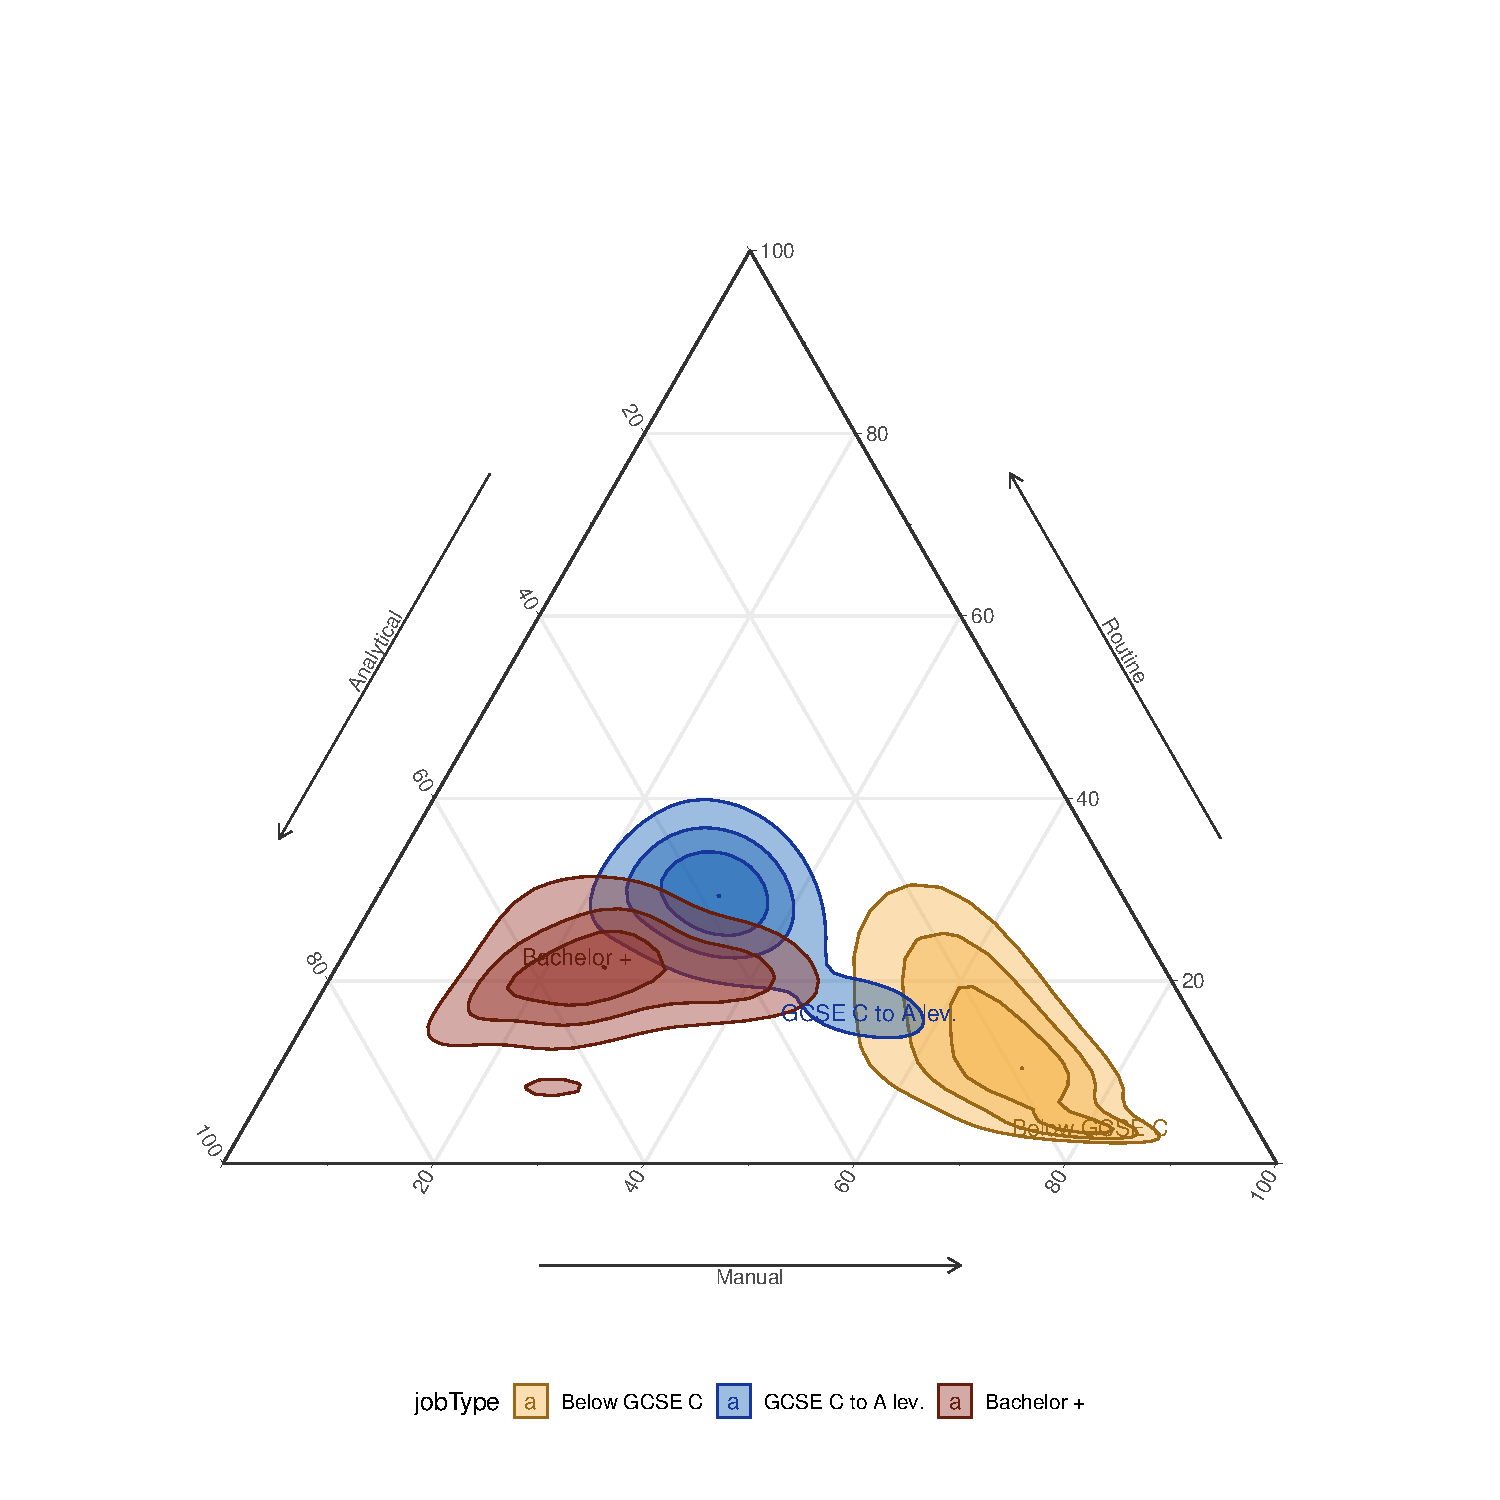
\includegraphics[width=.5\textwidth]{../output/densitySepDensityDum}} \subfloat[$ \sqrt{d_1d_2}\times observations_{LFS} $]{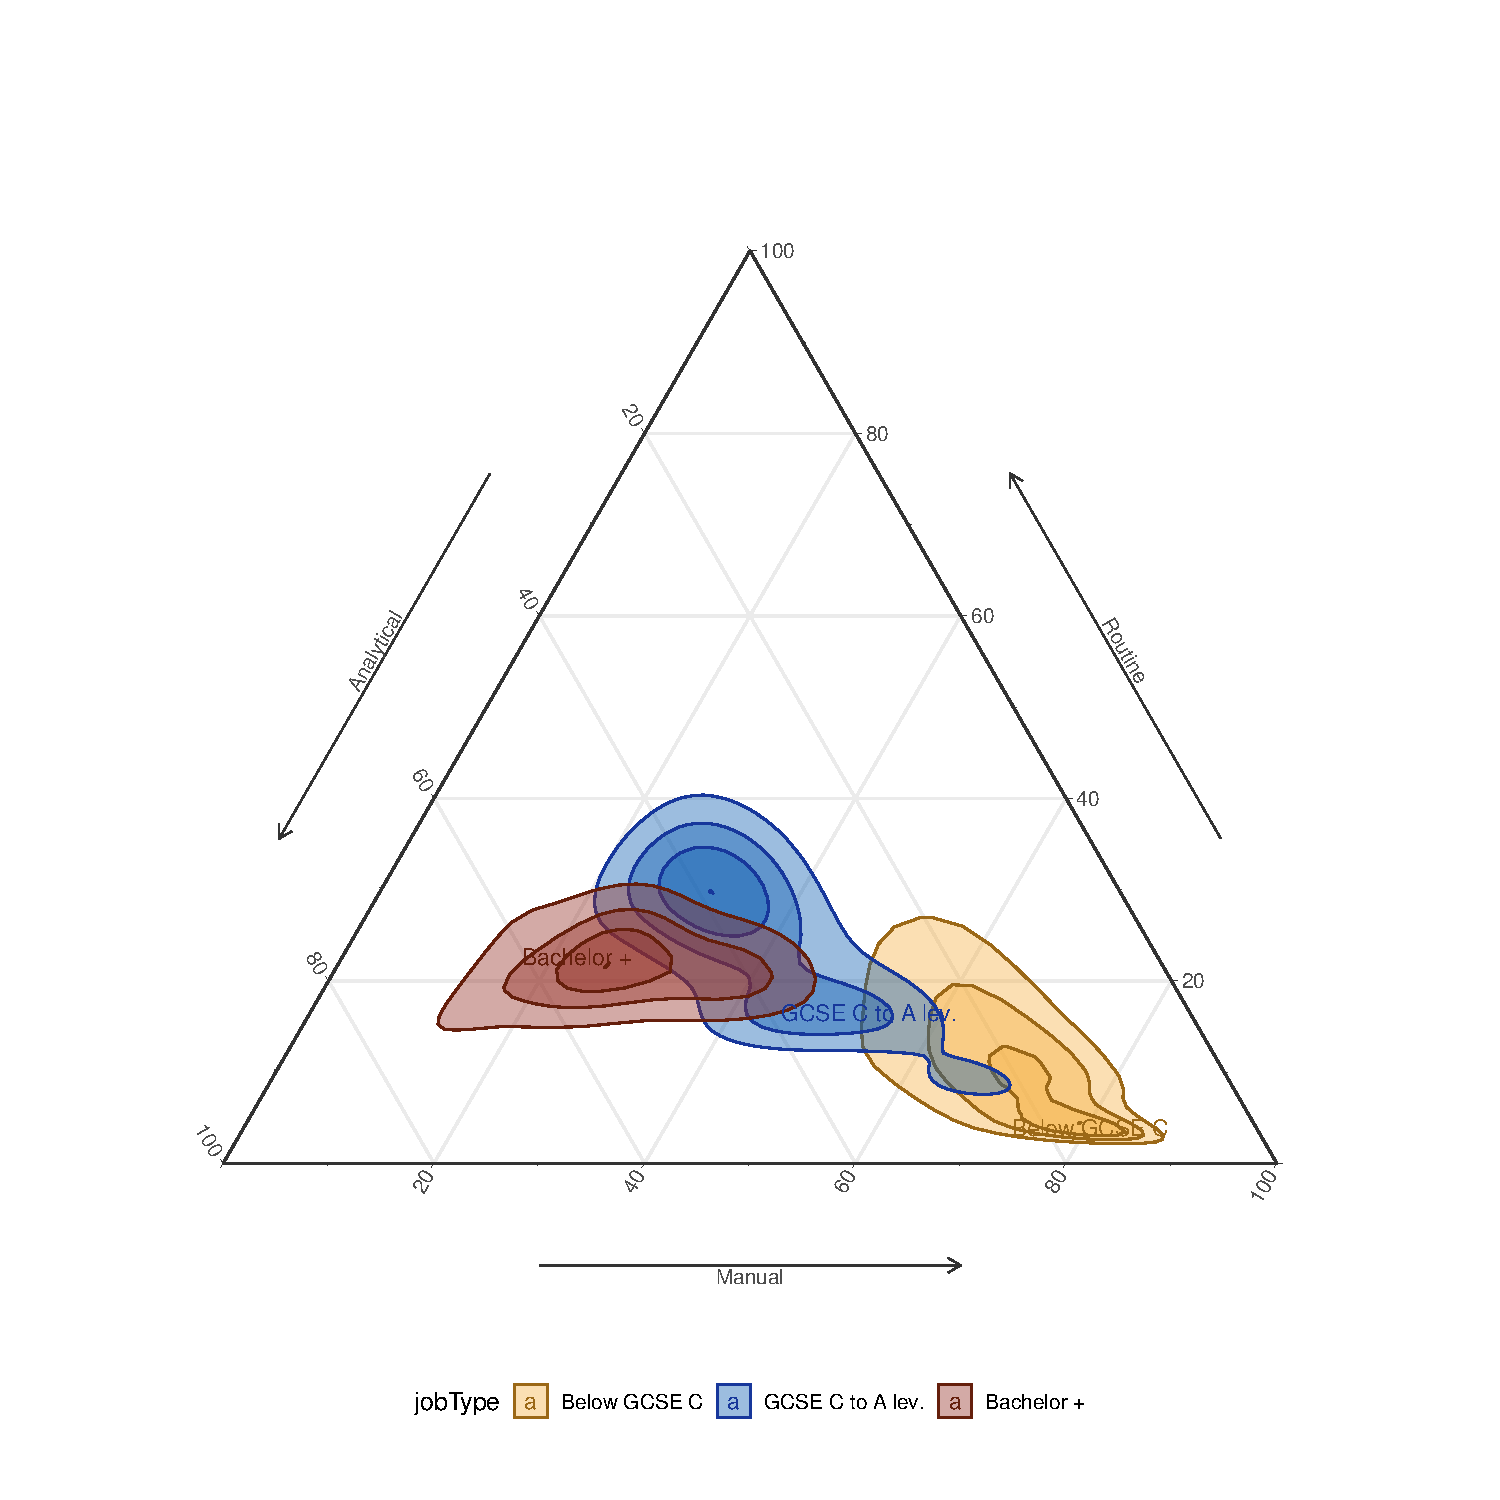
\includegraphics[width=.5\textwidth]{../output/densitySepDensityDumLFS1}} \\ \subfloat[$ \sqrt{d_1d_2\times observations_{LFS} \times observations_{SES}} $]{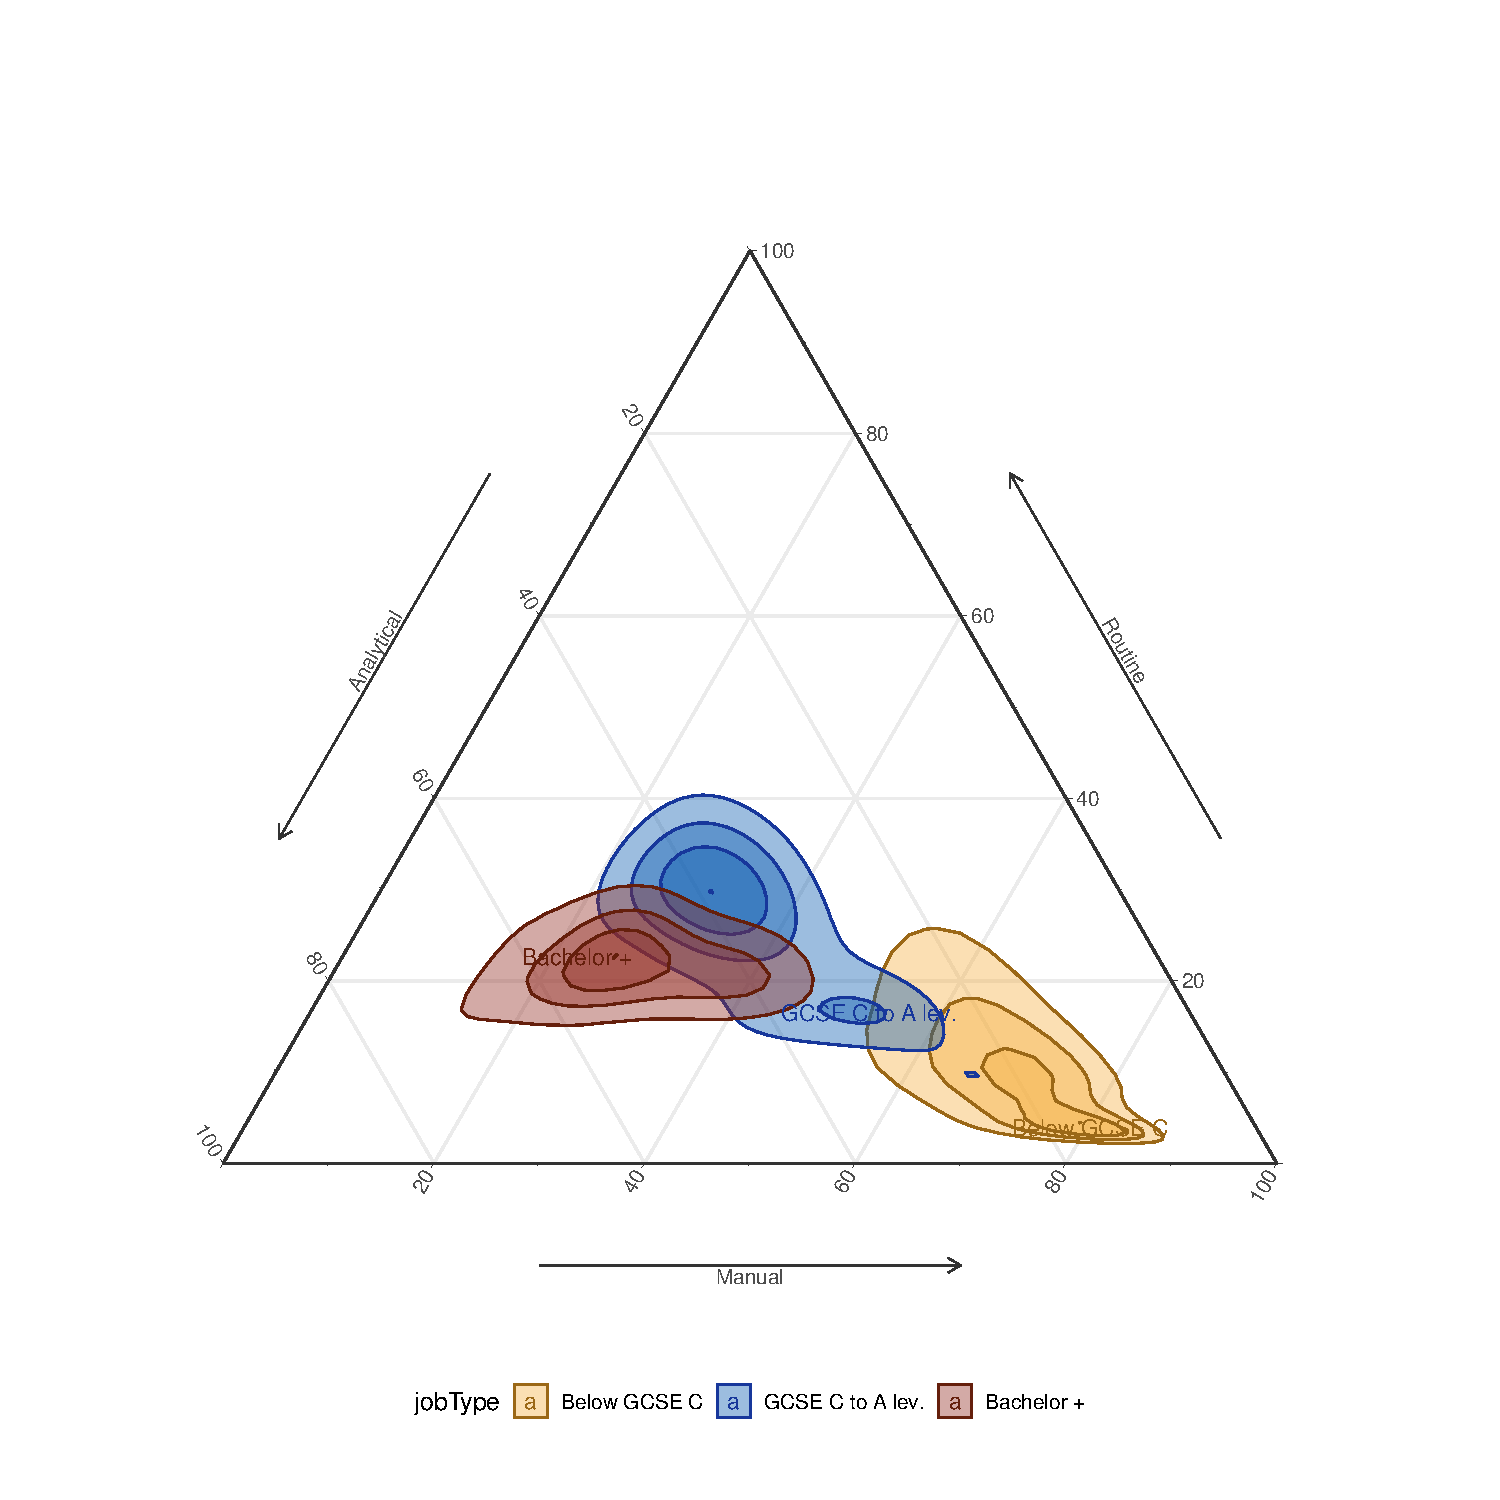
\includegraphics[width=.5\textwidth]{../output/densitySepDensityDumSES1}} \subfloat[$ \sqrt{d_1d_2}\times observations_{SES} $]{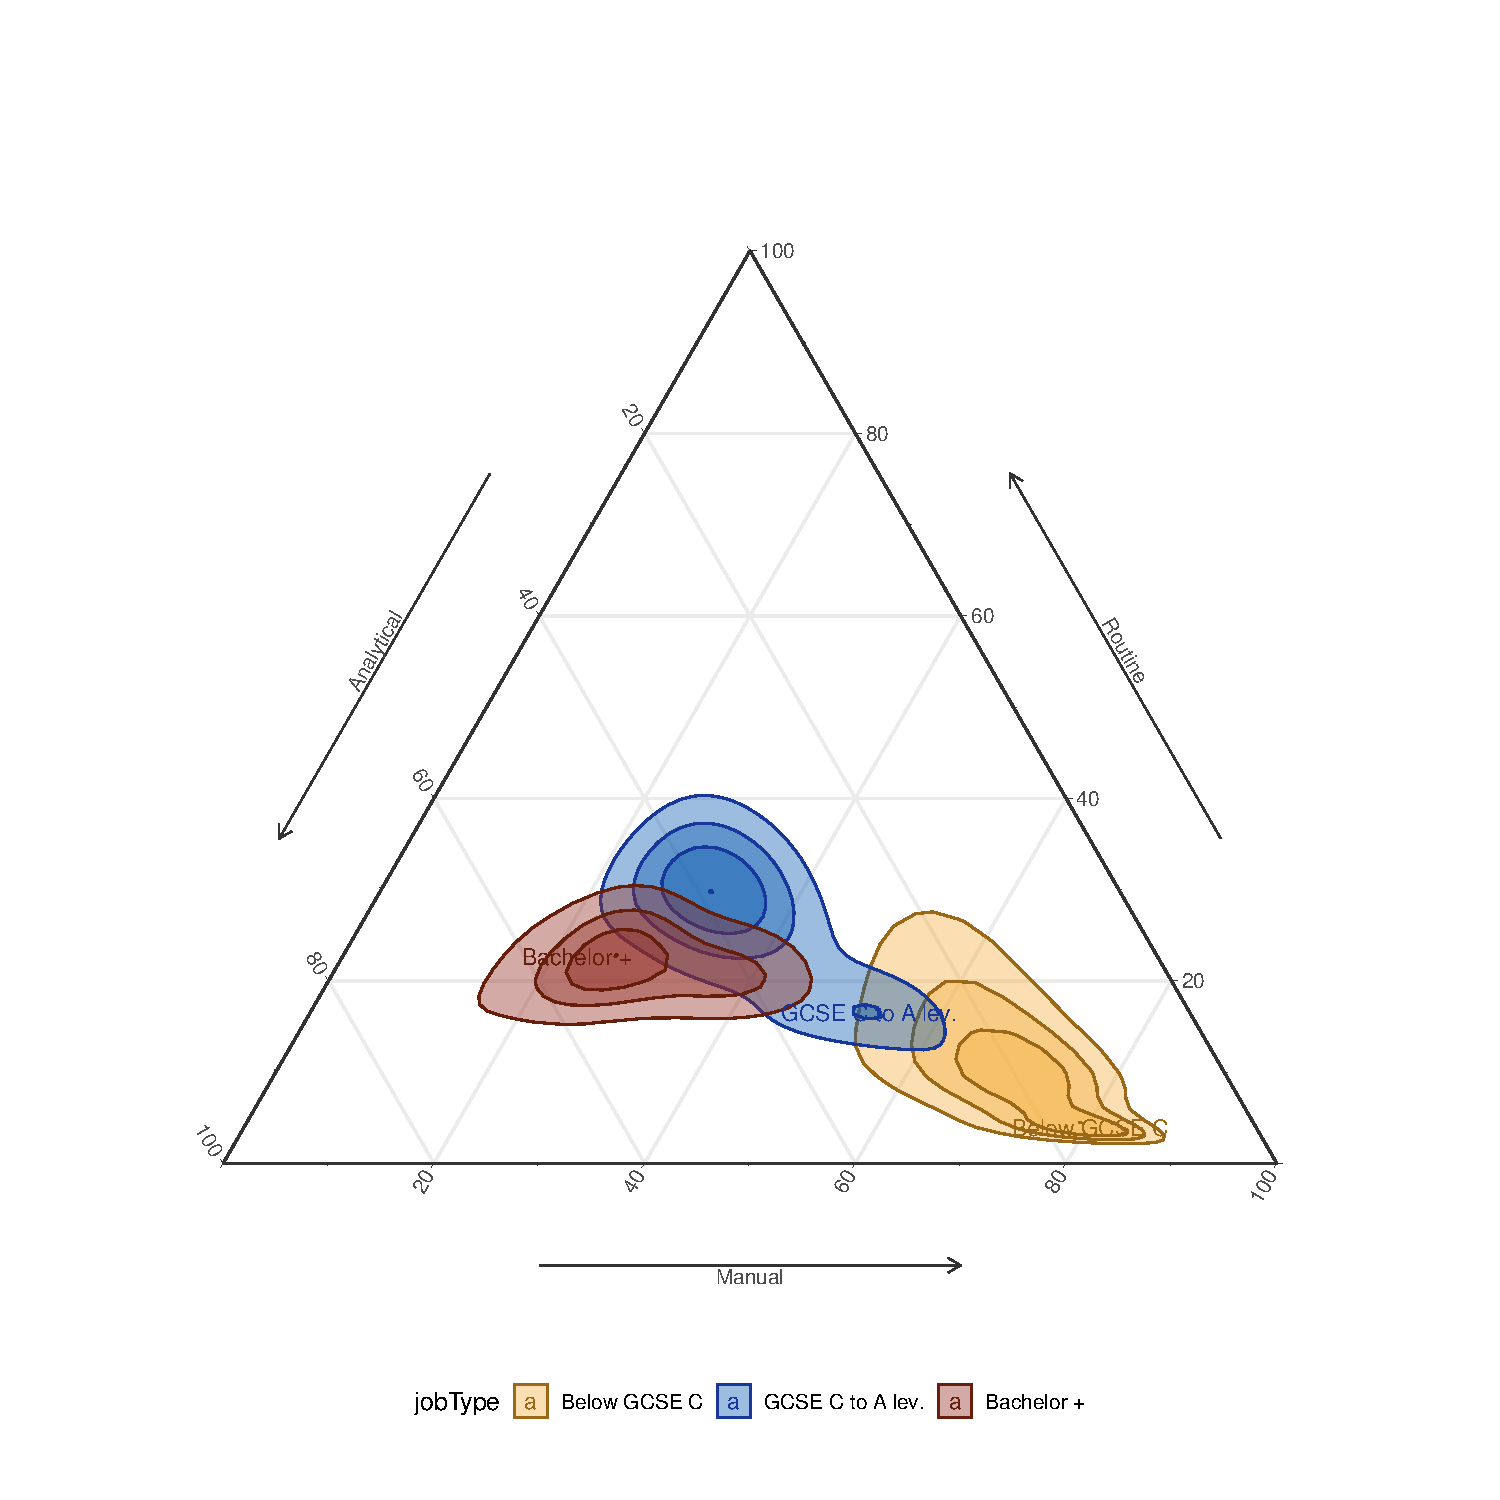
\includegraphics[width=.5\textwidth]{../output/densitySepDensityDumdistSES1}} \\ 
\par \begin{minipage}[h]{\textwidth}{\scriptsize\textbf{Note:} figure based on occupation-level averages. Figure generated on 15 Jun 2020 at 16:04:16. Figure generated using the dofile 3\_sesAnalysis/skillUseTriangles.do.}\end{minipage}
\end{figure}
